\section{Introduction}\label{sec:backstepping:introduction}
% \dropcap{C}{ontinuum} soft robots are systems entirely made of deformable materials, so to resemble the trunk of an elephant~\citep{della2020softencyclopedia}. 
% Controlling continuum soft robots is challenging because of the infinite amount of Degrees of Freedom (DoFs), the multi-body dynamics, nonlinear potentials, underactuation, and the high degree of uncertainties~\citep{george2018control}. 
% Combining feedback controllers % (inherently robust to model uncertainties)
% and simplified dynamical models can help taming this complexity and achieve good experimental performance \citep{thieffry2018control, della2020model, franco2021energy}.
%
%many approaches investigated the use of the constant curvature assumption and its extensions for static and dynamic control for continuum soft robotic manipulators~\citep{della2020model}.

%
%\citep{falkenhahn2014trajectory} proposes an optimal dynamic controller for pneumatically actuated manipulators which estimates an optimal trajectory that reduces the transition time and actuator jerk. Similarly, \citep{marchese2016dynamics} describes a trajectory optimization scheme for a soft planar manipulator. Clearly, there is need to not only incorporate the actuator dynamics into the trajectory planning, but also in the actual joint control. 

% Related work
% types of fluidic actuators

%While the actuator dynamics are often negligible for tendon-driven robots, the actuator dynamics of pneumatic actuators are slower and more nonlinear~\citep{george2018control}. 

% modeling
\dropcap{A}ccurate low-dimensional models of the continuum dynamics have been thoroughly investigated in recent years~\citep{faure2012sofa, grazioso2019geometrically, sadati2021tmtdyn}, serving as the base for model-based controllers \citep{boyer2020dynamics, della2023model}. 
In comparison, researchers have devoted little or no attention to modeling the actuator dynamics, despite this being far from a negligible effect in practice, in particular for pneumatic actuation. %Consider for example pneumatic actuation \citep{x}. 
%Simplified linear models 
%To the best of the authors' knowledge, the only work explicitly dealing with this challenge is \citep{wang2017soft}, which proposes a simplified model for a soft robotic gripper.
%
% In contrast, fewer publications investigate the modeling of the kinematics and dynamics of the mapping from actuation to configuration space. \citep{wang2017soft} proposes a simplified dynamic model for soft robotic grippers by considering the  deformation in a two-dimensional plane and dividing the Fluidic Elastomer Actuator (FEA) into a sequence of $n$ line segments with constant length. Viscoelastic joints are used to connect the segments with the bending motion generated by chamber expansion modeled by a series of rotational torques acting on each joint. The Euler-Lagrangian equation is used to derive the dynamics of the system of segments.  Experiments show a almost linear relationship between applied air pressure and bending angles for some FEAs while other FEAs incorporate slight nonlinear behaviours~\citep{wang2017soft}.
%
%Fluidic drive cylinders can have certain advantages over other fluidic energy supplies such as solenoid valves as for the fact that the segment curvature is monotonically related to the cylinder displacement, there is no exchange of fluid with the environment and the fluid flow can be continuously adjusted~\citep{marchese2016design}.
%
% PID controllers
The lack of models pairs with the scarcity of model-based dynamic controllers. Existing strategies only rarely reason on the actuators' dynamics, if not through simple heuristics.
%
For example, \citep{marchese2016design, della2020model} use a combination of PID control and inversion of quasi-static linear approximations to compensate for the actuators' dynamics. % more citations: lindenroth2016stiffness
%
This strategy may present clear limitations in terms of performance and stability assessment.
%
%to relate the desired torque in configuration space $\Bar{\tau}$ to a commanded actuation sequence of solenoid valves or to the actuation of pneumatic pistons. %A cascaded control approach is applied with an inner PID loop controlling pistons, and an outer loop controlling the curvature of the arm in~\citep{marchese2014design}. 
%
% Even when PID controllers work, well %because of the mostly linear relationship between chamber pressure and robot configuration for a limited pressure range~\citep{lindenroth2016stiffness}, 
% the gains are intricate to tune, and sensitive to changes in the robot design or actuator parameters.
%
% As an alternative, Gillespie et al.~\citep{gillespie2016simultaneous} propose a data-driven approach combined with an MPC controller.
% This sometimes works reasonably well as some experiments show a mostly linear relationship between chamber pressure and robot configuration for a limited pressure range~\citep{lindenroth2016stiffness}.
% 
% Marchese et al.~\citep{marchese2014design, marchese2016design} models the the dynamics of a pneumatic drive cylinder and the relationship between the change in fluid pressure inside the chambers of the arm segment and the pressure in the fluidic drive cylinder as a parameter of wall resistance and the compliance of elastomeric channels. Further, they also model the force output of an electric linear actuator to drive the fluidic cylinder dependent on the input motor voltage. This model however, is not used for control purposes and their controller relies on a cascaded control feedback algorithm with an inner PID loop running at \SI{1}{kHz} to control the position of the linear actuator and an outer loop executed at \SI{20}{Hz} to control the curvature of the arm segment by adapting the demanded piston position~\citep{marchese2014design}.

% sliding mode controller
% Sliding mode controllers based on second order lumped system dynamics have been explored to control a soft pneumatic actuator through the means of solenoid valves~\citep{skorina2015feedforward}. 
% The sliding mode controller was bench-marked against an additional feedforward term. The sliding mode controller together with the feedforward term shows the best tracking performance.

\begin{figure}[t]
  \centering
  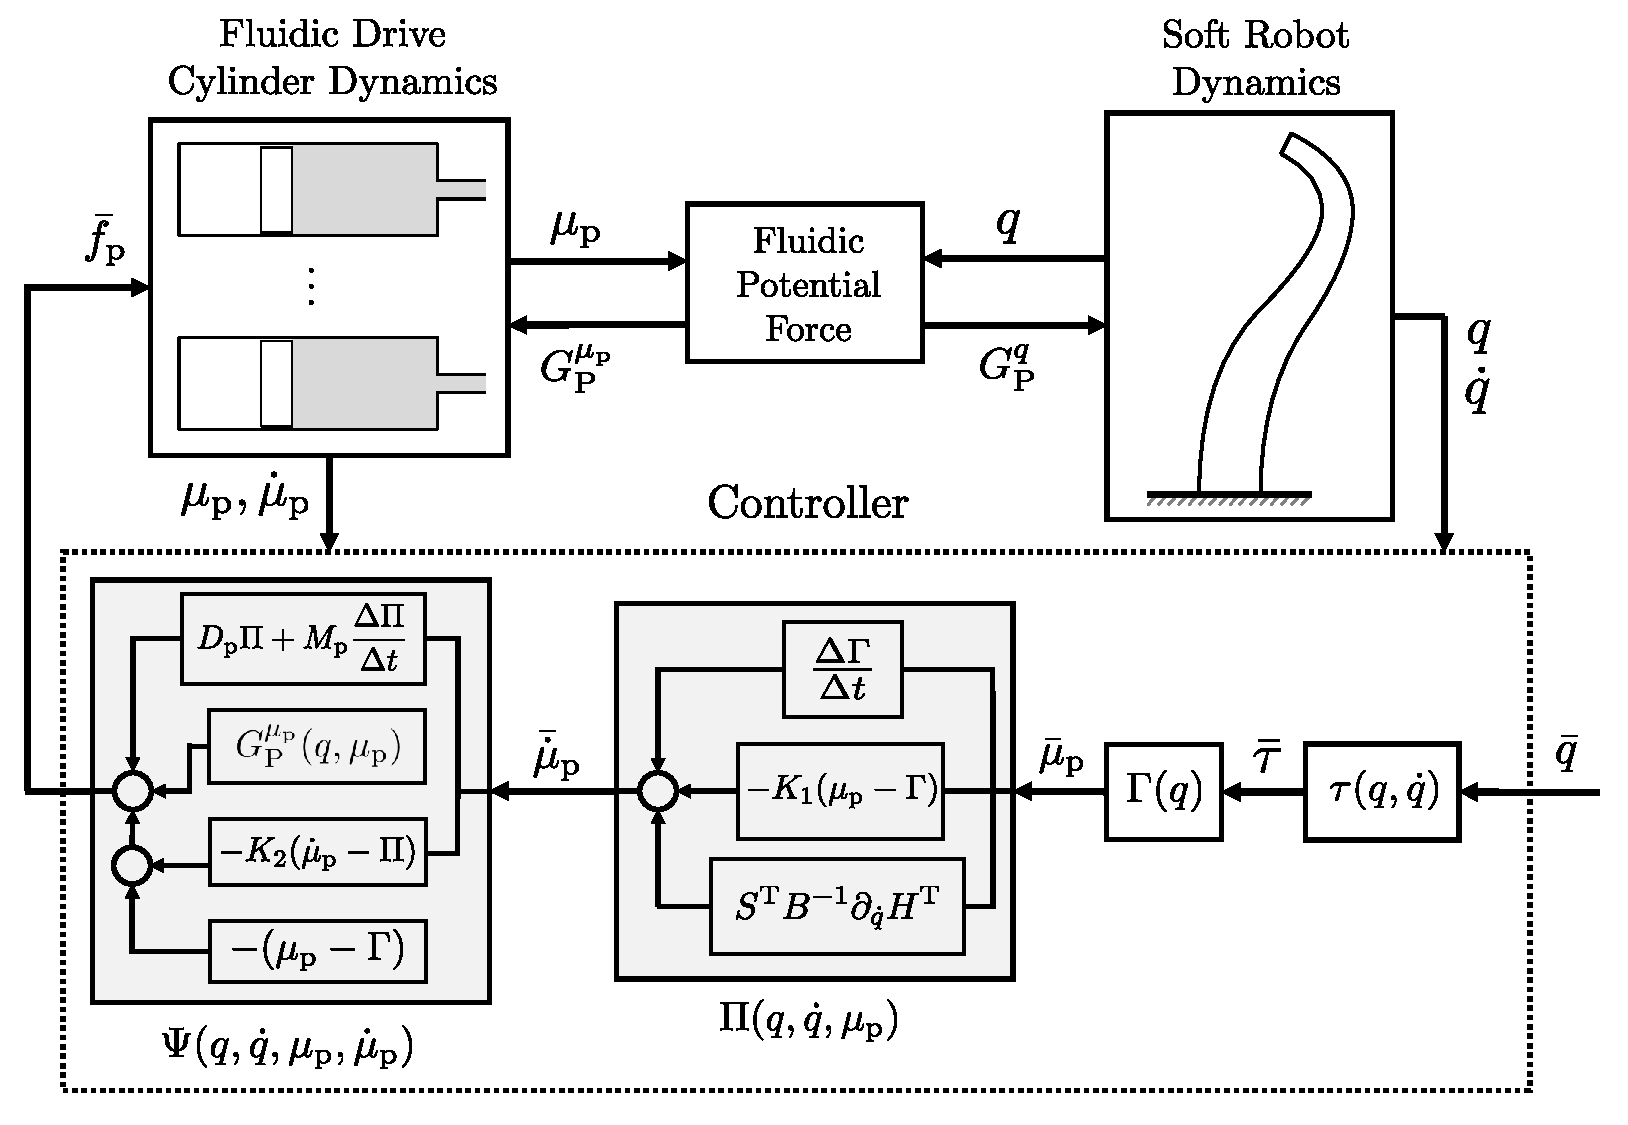
\includegraphics[width=0.9\columnwidth]{backstepping/figures/backstepping_graphics_control_scheme_v3_cropped.pdf}
  \caption{Schematic block diagram of the proposed nonlinear backstepping controller for a pneumatically-actuated soft robot. The approach considers both the fluidic drive cylinder and the soft system dynamics. It is agnostic to the chosen soft system controller in configuration-space $\tau(q,\dot{q})$.}\label{fig:backstepping:control_scheme}
\end{figure}

As model-based control of soft robots becomes a mature discipline, the need for general ways of dealing with actuators' dynamics becomes more pressing. In this chapter we deal with this challenge by follow a backstepping approach - which is an established strategy to deal with dynamical systems with triangular structure. %We focus on piston-driven pneumatically-actuated soft robots.
%
A pneumatic model based on the ideal gas law is derived and the pneumatic actuation system is compensated in a quasi-static fashion in Falkenhahn et al.~\citep{falkenhahn2016dynamic}.
%
% Seminal works have dealt with underactuated robotic systems using backstepping, as non-holonomic robots in \citep{fierro1997control}, flexible joint robots in \citep{oh1999control}, a single pneumatic muscle actuator in \citep{carbonell2001nonlinear}, variable stiffness actuated robots in \citep{petit2015backstepping}.
%
% For cable-driven soft continuum robots, a dynamic model based on strain-parametrization is developed in \citep{boyer2020dynamics} and subsequently used for CT control exploiting the triangular differential structure between the torques on the robot configuration and the applied cable tensions.
% with a composite control law consisting of fast part damping the configuration dynamics around the equilibrium trajectory determined by the slow control component.
%
Recent work by Wang et al.~\citep{wang2019parameter} uses backstepping for control of a continuum soft bending arm. Although interesting, the work is limited because it targets a linear model of a single DoF.
Similarily, Franco et al.~\citep{franco2021nonlinear} derive an energy-based control scheme for pneumatic manipulators while using a backstepping-based controller for comparison purposes.
% 
%{In a separate work considering the control of the \gls{BHA}, a pneumatic model based on the ideal gas law is derived and the pneumatic actuation system is controlled using a feedback-linearization controller that can compensate for the nonlinearities of the model~\citep{falkenhahn2016dynamic}.
Both pieces of work focus on pneumatic actuation with valves and thus cannot be immediately applied to systems actuated with fluidic drive cylinders.

To conclude, this chapter targets the dynamic control of piston-driven pneumatic-actuated soft robots (see for example Fig.~\ref{fig:backstepping:fluidic_drive_cylinder},~\ref{fig:backstepping:pcc_case_overview}). 
We provide general strategies for (i) augmenting existing dynamic models of soft robots through a description of pneumatic actuation, (ii) controlling these systems via model-based feedback. 
% Note that the application of backstepping is made not trivial by the non affine nature of the potential coupling. 
As an example, we specialize the model to planar soft robots satisfying the \gls{PCC} assumption~\citep{della2020model} including the proposal of a kinematic model for the air volume in the chambers, and the controller to the set-point regulation of configuration. In this context, we also propose a simplified, potential coupling-aware PID-like controller. We provide simulations showing the effectiveness of both strategies.

% backstepping
% Some recent work by Wang et al.~\citep{wang2018design, wang2019parameter} uses backstepping for control of a continuum soft bending arm with one \gls{DoF} actuated by pneumatic solenoid valves. A second-order transfer function is used to describe the dynamic behaviour from the driving pneumatic pressure to the continuum soft bending arm.
%\textcolor{red}{TODO: Explicitely describe how our approach is different}
% \citep{wang2018design} and \citep{wang2019parameter} approximate the air dynamics of a pneumatic solenoid valves and identifies the parameters using least-squares fitting. A second-order transfer function is used to describe the dynamic behaviour from the driving pneumatic pressure to the continuum soft bending arm. This dynamic model of the pressure regulator is used to control a bending actuator with one degree of freedom via backstepping to the PVM signal of the valve. Experiments show a superior trajectory tracking performance compared to a PID controller.
% Backstepping with load observation is also used to control a hydraulically controlled excavator by to compute the desired hydraulic force for motion tracking~\citep{bao2020energy}.
% Recent work analytically derives the chamber length of a soft actuator with three degrees of freedom as a function of input pressure with a Neo-Hookean deformation model only considering the kinematics of the system~\citep{xie2020design}. This model is used for inverse kinematic control of the input pressure for demanded azimuth and bending angles. Experiments to verify the analytical kinematic model show a considerable underestimation of the real bending angle.

% trajectory planning
% The full modelled dynamics of a continuum soft robot arm can also be leveraged within trajectory planning algorithms for bracing and grabbing strategies~\citep{marchese2016dynamics}. The system is broken down into three subsystems consisting of the fluidic drive cylinders, fluidic elastomer actuators and the soft manipulator with parameters identified from experimental data.
% One can further leverage the full modelled dynamics of a continuum soft robotic arm for trajectory planning algorithms such as for bracing and grabbing strategies~\citep{marchese2016dynamics}. They derive the fluidic energy stored in the system including a component lost due to resistivity of the fluid transmission line and viscous fluid friction. A cubic relationship between internal chamber volume and generalized torque on the system with a linear relationship between volume and bending angle is modelled and additionally a delay due to the impedance of the fluid transmission line introduced. The robotic arm is modelled with four fluidic drive cylinder pairs. The system is broken down into three subsystems consisting of fliudic drive cylinders, fluidic elastomer actuators mapping the cylinder displacements into generalized torques and the soft manipulator mapping the generalized torques into manipulator states. System identification techniques are used to identify the parameters of the modelled relationship between cylinder displacement and the generalized torques.

% contributions
%We state the contributions of this chapter as:
%
% To conclude, this chapter contributes to the state of the art in modeling and controlling soft robots with
% %
% \begin{itemize}
%     \item A strategy for including \textcolor{orange}{(Maxi) models of the actuation dynamics of pneumatically-driven soft robots into the control strategy. }
%     \item We propose a novel model-based, nonlinear and dynamic controller to pneumatically actuate fluidic drive cylinders in the framework of continuum soft robots. The approach is general and agnostic to the specific control strategy used for the soft manipulator.
%     \item We derive an analytical model for the volume in the pneumatic chambers of a continuum soft robot under \gls{PCC} assumption as a function of the configuration and subsequently develop a specialized controller for the \gls{PCC}-case.
% \end{itemize}